\documentclass[11pt]{article}
\usepackage[a4paper,margin=2.3cm]{geometry}
\usepackage{fontspec}
\setmainfont{Times New Roman}
\usepackage{polyglossia}
\setdefaultlanguage{romanian}
\usepackage{microtype}
\usepackage{booktabs}
\usepackage{graphicx}
\usepackage{eurosym}
\usepackage[hidelinks]{hyperref}
\usepackage{caption}
\usepackage{placeins}
\captionsetup{font=small,labelfont=bf}
\graphicspath{{figures/}}
\setlength{\parskip}{4pt}

\title{Cât de mult contează plafonul microîntreprinderilor?\\ \large Ce arată situațiile financiare ale tuturor firmelor din România, 2014--2025}
\author{Denis Siminiuc\thanks{Notă de politici bazată pe lucrarea „Bunching at a Moving Threshold: Firm Responses to Romania's Micro-Enterprise Tax, 2014--2025” (septembrie 2026). Lucrarea, codul și datele anonimizate sunt publice: \url{https://github.com/simdenis/romania-micro-enterprise-bunching}; date: doi:10.5281/zenodo.22863290. Redactarea și codul au fost realizate cu asistența unui model de limbaj (Anthropic Claude); alegerile de analiză, verificarea referințelor legale și a cifrelor și textul final sunt responsabilitatea autorului.}}
\date{Septembrie 2026}

\begin{document}
\maketitle

\section*{Pe scurt}

\begin{itemize}
\item Firmele se aglomerează imediat sub plafonul regimului de microîntreprindere în fiecare an din 2014 până în 2025. Aglomerarea urmărește plafonul când acesta se mută și cursul BNR când plafonul rămâne fix. Nu este un efect al rotunjirii: nimeni nu raportează din întâmplare o cifră de afaceri de 4.779.300 lei, iar vârful se mută la 4.869.400 lei în anul următor.
\item Local, efectul este mare: 2--8\% dintre firmele aflate la $\pm$20\% de plafon stau chiar sub el. La nivelul economiei este mic: 0,06--0,30\% din totalul firmelor care depun situații financiare. Costul bugetar al regimului vine de la sutele de mii de firme aflate mult sub plafon, nu de la cele câteva mii care se țin sub el.
\item Reacția vine din serviciile cu marje mari. În 2023, aglomerarea a fost de 12--15\% în serviciile profesionale, administrative, de sănătate și imobiliare și de 10\% în IT, față de 5\% în comerț, 3,5\% în transporturi și 1\% în agricultură.
\item Baza de impozitare schimbă ce raportează firmele. Firmele mutate în 2018 de la impozit pe profit la impozit pe venit, fără nicio acțiune proprie, au raportat marje mai mari cu circa 0,7 puncte procentuale; cele mutate înapoi în 2023 au raportat marje mai mici cu 1--2 puncte.
\item Condiția unui angajat din 2023 a dublat, în anul adoptării, rata la care firmele fără angajați au angajat exact o persoană: circa 20.000 de firme în plus. Dintre firmele care nu au angajat până la termen, patru cincimi au ieșit din regim.
\end{itemize}

\section{Ce s-a măsurat}

Regimul de microîntreprindere înlocuiește impozitul pe profit de 16\% cu un impozit de 1--3\% pe venituri pentru firmele cu venituri sub un plafon exprimat în euro. Plafonul s-a mutat de șase ori: 65.000 euro până în 2015, 100.000 în 2016, 500.000 în 2017, 1.000.000 în 2018--2022, 500.000 în 2023--2024, 250.000 în 2025 și 100.000 din 2026. Am folosit indicatorii din situațiile financiare anuale ale tuturor firmelor, publicați de Ministerul Finanțelor pe data.gov.ro (9,6 milioane de observații firmă-an), registrul plătitorilor ANAF pentru regimul fiscal al fiecărei firme și registrul comerțului pentru administratori și adrese.

Întrebarea de bază este simplă: câte firme raportează venituri chiar sub plafon, peste ce s-ar vedea dacă plafonul nu ar exista? Dificultatea obișnuită este că distribuția „fără plafon” trebuie ghicită. Aici nu trebuie: pentru că plafonul s-a mutat, fiecare nivel care a fost plafon într-un an a fost un punct obișnuit al distribuției în alți ani, iar acei ani servesc drept comparație. Metoda dă zero la 77 de locații fără plafon, ceea ce este testul ei de bună funcționare.

\section{Aglomerarea urmărește plafonul și cursul}

\begin{figure}[!htb]\centering
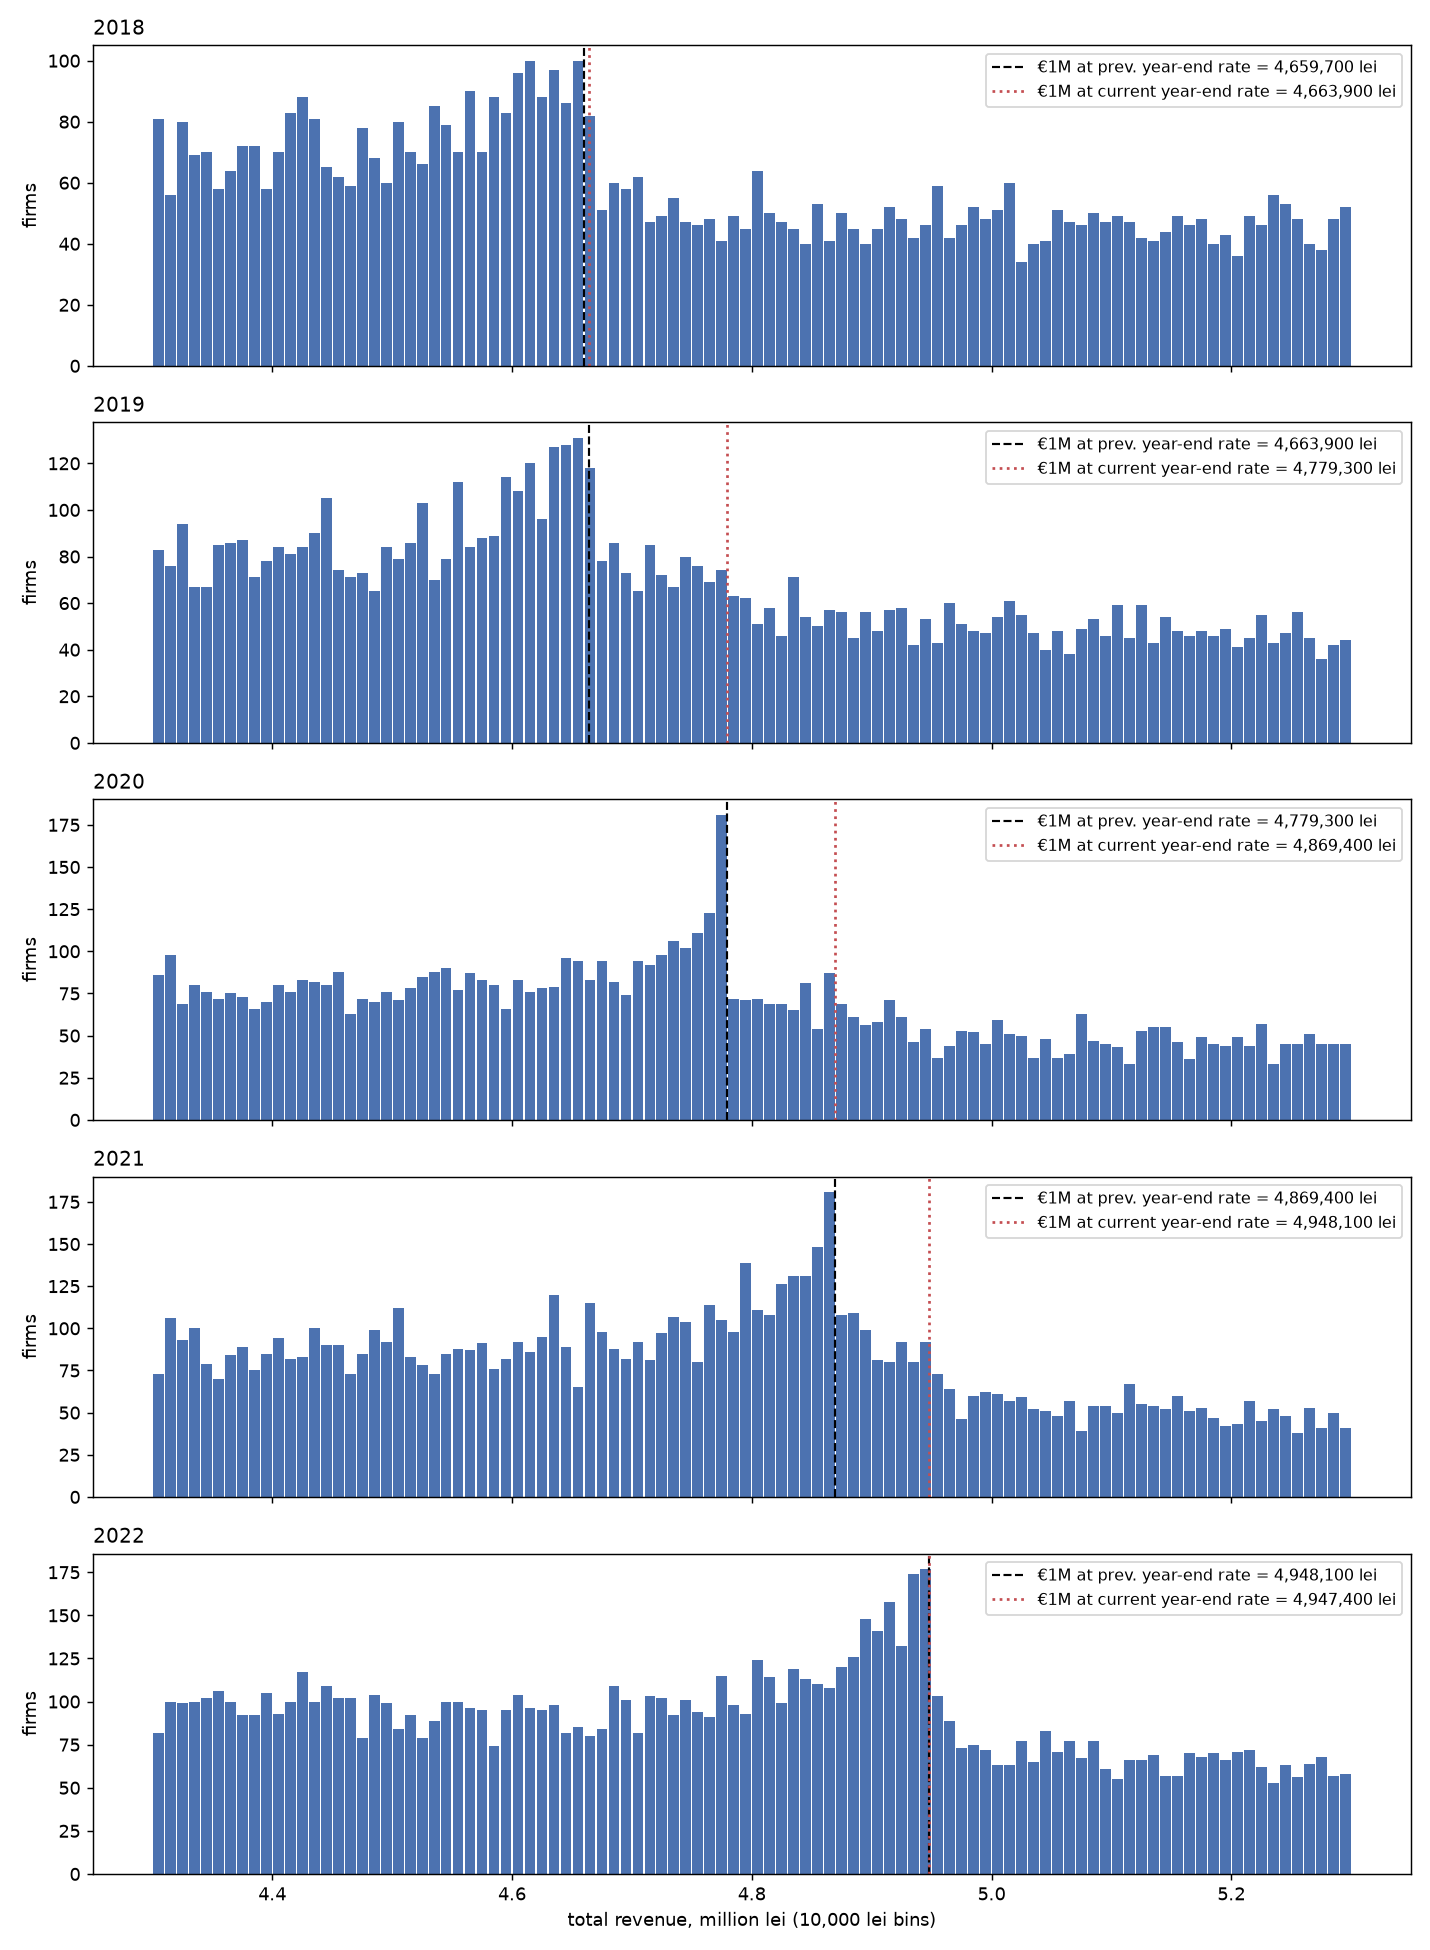
\includegraphics[width=0.85\textwidth]{lei_tracking_1M_2018_2022.png}
\caption{Venituri totale în lei în jurul echivalentului a 1.000.000 euro, 2018--2022, intervale de 10.000 lei. Linia întreruptă: plafonul la cursul BNR de la sfârșitul anului precedent; linia punctată: la cursul de la sfârșitul anului curent.}
\end{figure}

Între 2018 și 2022 plafonul a rămas 1.000.000 euro, dar valoarea lui în lei a crescut de la 4,66 la 4,95 milioane pe măsură ce leul s-a depreciat. Vârful distribuției veniturilor s-a mutat odată cu el, an de an, și stă la 1.400--5.600 lei sub valoarea plafonului la cursul de la sfârșitul anului precedent, cursul pe care legea îl prevede pentru testul din timpul anului. Când plafonul s-a schimbat, vârful s-a mutat la noul plafon: 65.000, 100.000, 500.000, 1.000.000, 500.000 și 250.000 euro. Când o reducere viitoare a fost adoptată, sau anunțată și apoi amânată, apare un al doilea vârf la plafonul viitor: în 2022 la 500.000 euro și în 2025 la 100.000 euro.

\section{Mare local, mic în agregat}

\begin{table}[!htb]\centering\small
\caption{Excesul de firme sub plafon, 2014--2025}
\begin{tabular}{lrrr}\toprule
An și plafon & Firme la $\pm$20\% de plafon & Exces de firme & Exces, \% din toate firmele \\ \midrule
2014, 65.000 € & 33.859 & 986 & 0,20 \\
2016, 100.000 € & 32.891 & 1.321 & 0,25 \\
2017, 500.000 € & 17.172 & 332 & 0,06 \\
2021, 1.000.000 € & 14.394 & 793 & 0,13 \\
2023, 500.000 € & 28.379 & 2.151 & 0,30 \\
2024, 500.000 € & 28.619 & 1.179 & 0,15 \\
2025, 250.000 € & 37.048 & 690 & 0,09 \\ \bottomrule
\end{tabular}
\begin{minipage}{0.95\linewidth}\vspace{2pt}\footnotesize Excesul de firme în intervalul de 5\% de sub plafon, față de distribuția din anii fără plafon în acel punct. Toate cele 14 estimări sunt în lucrare.\end{minipage}
\end{table}

Cel mai mare răspuns a fost în 2023, când plafonul s-a înjumătățit și ieșirea din regim a devenit definitivă: 7,6\% dintre firmele aflate la $\pm$20\% de plafon stăteau chiar sub el. Dar chiar și atunci excesul a fost de 2.151 de firme, 0,30\% din cele aproape 900.000 de firme care au depus situații financiare. Cifra de reținut pentru dezbaterea bugetară este aceasta: reacția la plafon este vizibilă, dar costul regimului nu stă acolo.

\section{Cine se aglomerează}

Regimul este avantajos doar pentru firmele cu marjă de profit peste raportul dintre cele două cote: 6,25\% la cota de 1\% și 18,75\% la cota de 3\%. Firmele aflate imediat sub plafon raportează marje mediane de 11--20\%, față de 6--10\% pentru cele imediat deasupra. Pe sectoare, aglomerarea din 2023 arată astfel:

\begin{table}[!htb]\centering\small
\caption{Aglomerarea sub plafonul de 500.000 euro în 2023, pe secțiuni CAEN}
\begin{tabular}{lrr}\toprule
Sector & Exces, \% din firmele la $\pm$20\% & Marja mediană a firmelor de sub plafon \\ \midrule
Servicii profesionale & 14,8 & 0,39 \\
Servicii administrative & 13,3 & 0,29 \\
Construcții & 12,6 & 0,25 \\
Sănătate & 12,0 & 0,32 \\
Imobiliare & 11,2 & 0,43 \\
IT și comunicații & 10,1 & 0,34 \\
Industrie prelucrătoare & 6,5 & 0,16 \\
Comerț & 4,8 & 0,12 \\
Transporturi & 3,5 & 0,10 \\
Agricultură & 1,0 & 0,08 \\
HoReCa (fără plafon în 2023) & 0,9 & 0,14 \\ \bottomrule
\end{tabular}
\end{table}

Sectoarele care se aglomerează sunt exact cele vizate de modificările din 2023--2024 și cele în care regimul economisește cel mai mult impozit pe fiecare leu de venit.

\section{Baza de impozitare schimbă ce raportează firmele}

O microîntreprindere plătește același impozit indiferent de profitul raportat; o firmă pe impozit pe profit nu. Schimbările de plafon permit un test direct. În 2018, plafonul a crescut de la 500.000 la 1.000.000 euro, astfel că firmele cu venituri între aceste valori au fost mutate de pe impozit pe profit pe impozit pe venit fără nicio acțiune proprie; în 2023, reducerea le-a mutat înapoi. Comparate cu firme de aceeași mărime rămase pe impozit pe profit, firmele mutate în regim în 2018 au raportat marje mai mari cu 0,7 puncte în primul an, iar cele mutate afară în 2023 au raportat marje mai mici cu 1,0, 1,6 și 2,0 puncte în trei ani, de la o bază de circa 6\%. Efectul de ieșire este cel robust; cel de intrare este semnificativ doar în primul an. Interpretarea: sub impozitul pe profit, o parte din costuri sunt raportate cu ochii la impozit.

\section{Condiția unui angajat}

Din 2023, o microîntreprindere trebuie să aibă cel puțin un angajat, condiție testată la 31 decembrie 2022 și adoptată în iulie 2022. Dintre firmele mici fără angajați, 22,3\% au trecut la exact un angajat în 2022, față de 11,1--11,3\% în anii precedenți; printre firmele mari, neafectate de regulă, rata a rămas la 5--6\%. Sunt circa 20.000 de firme cu un angajat în plus. Dintre microîntreprinderile care nu aveau niciun angajat la sfârșitul lui 2022, 82\% erau înregistrate la impozit pe profit în 2023 și doar 15\% aveau un angajat până la sfârșitul lui 2023. Angajările au venit în anul adoptării; cine nu a angajat până la termen a ieșit din regim. Câmpul din situațiile financiare este numărul mediu de salariați, deci un contract cu timp parțial contează ca un angajat; citim rezultatul ca respectare a condiției la costul minim, nu ca locuri de muncă noi.

\section{Două rezultate secundare}

\textbf{Pragul de TVA.} Firmele se aglomerează și mai puternic sub pragul de scutire de TVA, de 220.000 și apoi 300.000 lei. Când pragul a urcat la 395.000 lei la 1 septembrie 2025, vârful de la 300.000 a dispărut din distribuția anului 2025 și a apărut unul la 395.000: firmele și-au ajustat cifra de afaceri anuală la un prag schimbat cu patru luni înainte de sfârșitul anului. Odată mutat pragul de TVA, se vede și pragul de 60.000 euro dintre cotele de 1\% și 3\%: firmele reacționează la el, dar de circa cinci ori mai slab decât la pragul de TVA.

\textbf{Divizarea firmelor.} Firmele de sub plafon au, ceva mai des decât firmele de aceeași mărime și vârstă de deasupra lui, un administrator care a înregistrat o altă firmă în ultimele 18 luni (2,7\% față de 2,0\%). Dar veniturile cumulate ale firmelor cu același administrator nu se aglomerează la 500.000 euro în 2024, când legea a început să testeze plafonul pe firme legate. Tratăm divizarea ca o corelație, nu ca un mecanism dovedit; datele deschise nu conțin asociații, ci doar administratorii.

\section{Ce înseamnă pentru politici}

\begin{enumerate}
\item \textbf{Plafonul este o preocupare de ordinul doi.} Mutarea lui schimbă comportamentul câtorva mii de firme; costul bugetar și distorsiunile regimului vin de la firmele intramarginale. Simulările statice de venituri, care presupun că firmele nu reacționează, nu greșesc cu mult tocmai din acest motiv.
\item \textbf{Regimul avantajează serviciile cu marje mari.} Lista de activități taxate cu 3\% indiferent de venit merge în direcția corectă, dar este departe de a acoperi sectoarele care se aglomerează cel mai mult.
\item \textbf{Condițiile secundare produc conformare la cost minim.} Condiția unui angajat a produs contracte, nu neapărat locuri de muncă; testarea plafonului pe firme legate nu a produs, în primul an, aglomerare a veniturilor cumulate.
\item \textbf{Baza de impozitare contează pentru ce se raportează.} Marjele raportate cresc când firma trece pe impozit pe venit și scad când revine pe impozit pe profit; orice analiză a profitabilității firmelor mici trebuie să țină cont de regimul lor fiscal.
\end{enumerate}

\FloatBarrier
\end{document}
